\documentclass[10pt]{beamer}
\usepackage{graphicx}
\usepackage{amsmath}
\usepackage{bm}
\usepackage{hyperref}
\usepackage{booktabs}
\usepackage{color}
\usepackage{xcolor}
\usepackage{amssymb}      % For \checkmark
\usepackage[utf8]{inputenc} % For ° and £ (or use \pounds)
\usepackage{tikz}
\usetikzlibrary{shapes.geometric, arrows, positioning, calc, fit, backgrounds}

% Enable speaker notes (uncomment one of these options)
%\setbeameroption{show notes} % Notes on separate pages
\setbeameroption{show notes on second screen=right} % Notes on second screen for presentation
\usepackage{pgfpages}

% TikZ styles for block diagrams
\tikzstyle{startstop} = [rectangle, rounded corners, minimum width=3cm, minimum height=1cm,text centered, draw=black, fill=red!30]
\tikzstyle{process} = [rectangle, minimum width=3cm, minimum height=1cm, text centered, text width=3cm, draw=black, fill=blue!20]
\tikzstyle{sensor} = [rectangle, minimum width=2.5cm, minimum height=0.8cm, text centered, text width=2.5cm, draw=black, fill=green!20]
\tikzstyle{power} = [rectangle, minimum width=2.5cm, minimum height=0.8cm, text centered, text width=2.5cm, draw=black, fill=yellow!30]
\tikzstyle{arrow} = [thick,->,>=stealth]

\usetheme{Boadilla}

\title{Free-Roving Subsea Cable Inspection Drone}
\subtitle{A Technical Feasibility Study}
\author{Jerry Liu (yhl63) \\ Zihe Liu (zl559)}
\institute{University of Cambridge}
\date{\today}

% Custom footnote settings
\setbeamercolor{footline}{use=structure,bg=structure.fg, fg=white}
\setbeamertemplate{footline}{%
  \leavevmode%
  \begin{beamercolorbox}[wd=\paperwidth,ht=2.5ex,dp=1ex]{footline}%
    \hfill
    \insertshorttitle
    \hfill
    \insertframenumber/\inserttotalframenumber
    \hspace{1em}
  \end{beamercolorbox}%
}

% Add section divider slides
\AtBeginSection{
  \begin{frame}
  \vfill
  \centering
  \begin{beamercolorbox}[sep=8pt,center,shadow=true,rounded=true]{title}
    \usebeamerfont{title}\insertsectionhead\par%
  \end{beamercolorbox}
  \vfill
  \end{frame}
}

\begin{document}

% Title slide
\frame{\titlepage}

%%%%%%%%%%%%%%%%%%%%%%%%%%%%%%%%%%%%%%%%%%%%%%%%%%%%%%%%%%%%%%%%%%%%%
\section{Problem - Subsea Cable Inspection}

\begin{frame}{Problem - Why Subsea Cables Matter}
  \begin{columns}[T]
    \begin{column}{0.45\textwidth}
      \textbf{Backbone of the Internet:}
      \begin{itemize}
        \item 97-99\% of intercontinental data traffic
        \item 500+ cables worldwide
        \item 14 million kilometers total
        \item 2-5 cm diameter (garden hose size)
      \end{itemize}
    \end{column}
    \begin{column}{0.52\textwidth}
      \includegraphics[width=\textwidth]{img/subsea_cables.png}
    \end{column}
  \end{columns}

  \note{Before we dive into our design and feasibility assessment, let's give some context to the problem we're tackling: Subsea cables. Your internet connection, whether that be for online banking or video calls, 97-99\% of that data goes through a dense network of over 500+ undersea cables, spanning a total of 14 million kilometers over the seafloor making it THE largest and possibly greatest man-made infrastructure ever. This is the backbone of the internet, and when they fail, the consequences are severe. Despite the significance of these cables, these cables are no thicker than your average garden-hose around 2-5 cm in diameter, with hair-thin strands of optical fiber embedded within, designed to remain undisturbed across the seabed.}
\end{frame}

\begin{frame}{Problem - Current Limitations}
  \begin{columns}[T]
    \begin{column}{0.55\textwidth}
      \includegraphics[width=\textwidth]{img/ship.png}
    \end{column}
    \begin{column}{0.42\textwidth}
      \textbf{Cable Faults:}
      \begin{itemize}
        \item ~200 faults/year
        \item Shallow waters most vulnerable
        \item Shetland Islands 2022: 23,000 people offline
      \end{itemize}

      \vspace{0.5em}

      \textbf{Traditional: Tethered ROVs}
      \begin{itemize}
        \item[+] Unlimited power
        \item[+] Real-time comms
        \item[--] Limited range
        \item[--] Tether entanglement
        \item[--] High operational cost
      \end{itemize}
    \end{column}
  \end{columns}

  \vspace{1em}
  \centering
  \textit{Solution: Free-roving Autonomous Underwater Vehicle}

  \note{In shallow waters however, these subsea cables are susceptible to a wider range of disturbances, largely from human activities such as anchoring, or snagged by nets, resulting in roughly 200 faults a year. In October 2022, both cables serving the Shetland Islands were damaged. For days, 23,000 people had no internet, could not use card payments, could not access online banking. Businesses lost thousands. Emergency services were disrupted. These are not rare events, they require constant monitoring and effective maintenance. When a fault occurs, an army of ships strategically placed around the world would identify and repair the location of the fault, which usually involves the usage of a tethered drone to inspect the damaged cable. Despite the effectiveness of tethered communications and unlimited power, this comes at the cost of a limited range of motion and risks of entanglement, as well as higher maintenance costs for dedicated vessels. Therefore we propose the use of an untethered AUV}
\end{frame}


%%%%%%%%%%%%%%%%%%%%%%%%%%%%%%%%%%%%%%%%%%%%%%%%%%%%%%%%%%%%%%%%%%%%%
\section{Requirements and Operating Environment}

\begin{frame}{Requirements and Operating Environment}
  \textit{``A free-roving (no umbilical cable) submarine inspection drone is required for undersea cables: operating down to 250 m depth. It should have an endurance of 2 hours continuously powered operation, carrying video and ultrasound imaging equipment drawing a 30 W electrical load, and have suitable propulsion to travel up to 4 m/s peak speed with 1 m/s cruise. Total mass is to be $<$ 25 kg, to allow easy handling on board the mothership.''}

  \vspace{0.5em}

  \begin{columns}[T]
    \begin{column}{0.48\textwidth}
      \textbf{Key Specifications:}
      \begin{itemize}
        \item Depth: 250m (25 bar pressure)
        \item Endurance: 2 hours continuous
        \item Speed: 1 m/s cruise, 4 m/s peak
        \item Payload: 30W (imaging + ultrasound + lighting)
        \item Mass: $<$ 25 kg total
      \end{itemize}
    \end{column}

    \begin{column}{0.48\textwidth}
      \textbf{Operating Challenges:}
      \begin{itemize}
        \item Pressure: $P = \rho gh \approx 25$ bar
        \item Temperature: ~4°C seawater
        \item No GPS/RF underwater
        \item Saltwater corrosion
        \item Turbid water (limited visibility)
      \end{itemize}
    \end{column}
  \end{columns}

  \note{At 250 m depth, the pressure is approximately 25 bar (2.5 MPa). This is calculated using P = rho g h, where rho is seawater density (1027 kg/m cubed), g is gravitational acceleration, and h is depth. The temperature is approximately 4 degrees Celsius. Materials must resist corrosion - we will use 316 stainless steel and anodized aluminum. Sensors must work in turbid water with near-zero visibility. Communications are limited to acoustic modems underwater since radio and GPS signals cannot penetrate seawater beyond a few meters. The 30W payload limit includes all imaging equipment (camera), ultrasound sensors, and lighting - this is a combined budget, not separate allocations.}
\end{frame}

%%%%%%%%%%%%%%%%%%%%%%%%%%%%%%%%%%%%%%%%%%%%%%%%%%%%%%%%%%%%%%%%%%%%%
\section{Existing Commercial Solutions}

\begin{frame}{Existing Commercial Solutions}
  \begin{table}
    \scriptsize
    \begin{tabular}{lcccccc}
      \toprule
      \textbf{Model}      & \textbf{Type} & \textbf{Mass} & \textbf{Depth} & \textbf{Speed} & \textbf{Endurance} & \textbf{Cost} \\
      \midrule
      \textbf{Our Target} & AUV           & $<$25 kg      & 250m           & 4 m/s peak     & 2 hrs              & \$10-23K      \\
      \midrule
      Iver3 (L3Harris)    & AUV           & 27-39 kg      & 100m           & 1.3 m/s        & 8-14 hrs           & \$75-120K     \\
      ecoSUB m-Power+     & AUV           & 17 kg         & 500m           & ~1.5 m/s       & 8-10 hrs           & £35-50K       \\
      Boxfish AUV         & AUV           & 25 kg         & 300-600m       & ~2 m/s         & 10 hrs             & \$80-150K     \\
      BlueROV2            & ROV           & 10-11 kg      & 100-300m       & 1 m/s          & 3-5 hrs            & \$3-3.5K      \\
      \bottomrule
    \end{tabular}
  \end{table}

  \vspace{0.3em}

  \begin{columns}[T]
    \begin{column}{0.24\textwidth}
      \centering
      \includegraphics[width=0.9\textwidth]{img/iver3.png}
      \tiny Iver3: Single thruster + fins
    \end{column}
    \begin{column}{0.24\textwidth}
      \centering
      \includegraphics[width=0.9\textwidth]{img/ecosub.png}
      \tiny ecoSUB: 500m rated, alkaline
    \end{column}
    \begin{column}{0.24\textwidth}
      \centering
      \includegraphics[width=0.9\textwidth]{img/boxfish.png}
      \tiny Boxfish: Tethered AUV, 6-DOF
    \end{column}
    \begin{column}{0.24\textwidth}
      \centering
      \includegraphics[width=0.9\textwidth]{img/bluerobtoicsROV2.png}
      \tiny BlueROV2: Tethered ROV, 6-DOF
    \end{column}
  \end{columns}

  \vspace{0.3em}
  \centering
  Key finding: No commercial AUV $<$25 kg achieves 4 m/s sustained speed

  \note{Many commercial solutions exist but vary in capability. Commercial designs such as the Iver3 and ecoSUB use fully autonomous operation with single thruster plus fins for pitch/yaw control. The Boxfish uses 8 vectored thrusters for full 6-DOF control including hovering. BlueROV2 is included as it is a Blue Robotics reference platform that proves component viability, though it is a tethered ROV not an autonomous AUV. Key finding: Few commercial AUVs under 25 kg achieve 4 m/s sustained speed - most operate at 1.5-2.5 m/s due to power limitations. Commercial pricing (50-150K dollars) reflects support and warranty, not just hardware costs. Our target specifications are ambitious but achievable with careful trade-off management.}
\end{frame}

%%%%%%%%%%%%%%%%%%%%%%%%%%%%%%%%%%%%%%%%%%%%%%%%%%%%%%%%%%%%%%%%%%%%%
\section{Design Approach and System Architecture}

\begin{frame}{Trade-offs}
  \begin{center}
    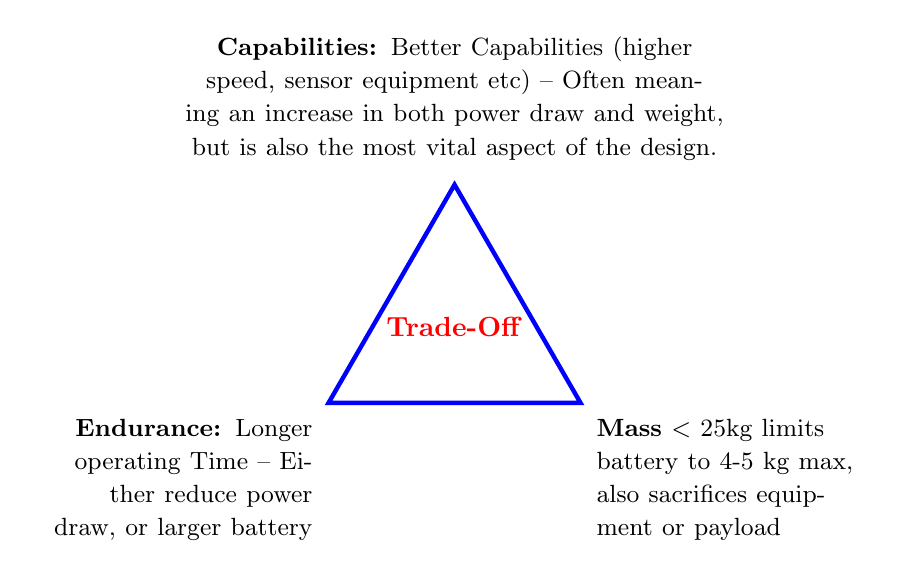
\begin{tikzpicture}[scale=0.8]
      % Triangle
      \draw[ultra thick, blue] (0,0) -- (4,0) -- (2,3.464) -- cycle;

      % Center text
      \node[text width=2.5cm, align=center] at (2,1.2) {
        \textcolor{red}{\textbf{Trade-Off}}
      };

      % CAPABILITIES (top vertex)
      \node[text width=8cm, align=center, anchor=south] at (2,3.7) {
        \small \textbf{Capabilities:} Better Capabilities (higher speed, sensor equipment etc) – Often meaning an increase in both power draw and weight, but is also the most vital aspect of the design.
      };

      % ENDURANCE (bottom left vertex)
      \node[text width=3.5cm, align=right, anchor=north east] at (-0.1,-0.1) {
        \small \textbf{Endurance:} Longer operating Time – Either reduce power draw, or larger battery
      };

      % MASS (bottom right vertex)
      \node[text width=3.5cm, align=left, anchor=north west] at (4.1,-0.1) {
        \small \textbf{Mass} $<$ 25kg limits battery to 4-5 kg max, also sacrifices equipment or payload
      };
    \end{tikzpicture}
  \end{center}

  \vspace{0.5em}
  \textbf{Our Solution:} \textit{Mission profile with 80\% cruise (1 m/s) + 20\% sprint (4 m/s)}
\end{frame}


\begin{frame}{System Design Directions}
  \begin{center}
    \begin{itemize}
      \item Autonomous/programmable solution to remove the need for high-quality real-time data transmission which limits untethered ROVs
            \begin{itemize}
              \item Enables self-contained operation with onboard power, navigation, and data handling
              \item Supports scalable inspection missions without reliance on surface tethers
            \end{itemize}

      \item 6-thruster design for stability and hovering capabilities for detailed inspection
            \begin{itemize}
              \item Provides full 6-DOF control for precise hovering, lateral motion, and pitch/yaw stability
              \item Redundancy for safe recovery in case of partial thruster failure
              \item Efficient low-speed maneuvering for inspection tasks
            \end{itemize}
      \item Hull design to be cylindrical (pill) shaped to minimise volume as well as simplify hydrodynamic calculations.
            \begin{itemize}
              \item Streamlined shape reduces drag forces at higher speeds
              \item Simplifies internal component layout and waterproofing
              \item Proven design in existing AUVs for balance of speed and stability
            \end{itemize}
    \end{itemize}
  \end{center}
\end{frame}

\begin{frame}{System Architecture - Simplified Block Diagram}
  \begin{center}
    \centering
    \includegraphics[width=0.9\textwidth]{img/System_design.png}

    % \begin{tikzpicture}[node distance=2.5cm, every node/.style={font=\small}]
    %   % Five main blocks in circular arrangement
    %   \node (power) [process, fill=yellow!30, minimum width=3.5cm, minimum height=1.2cm] {
    %     \textbf{POWER}\\
    %     3× 18Ah Li-ion\\
    %     799 Wh, 14.8V
    %   };

    %   \node (control) [process, fill=blue!30, right of=power, minimum width=3.5cm, minimum height=1.2cm] {
    %     \textbf{CONTROL}\\
    %     Navigator + RPi4\\
    %     IMU, Depth, GPS
    %   };

    %   \node (propulsion) [process, fill=green!30, below of=power, yshift=-0.5cm, minimum width=3.5cm, minimum height=1.2cm] {
    %     \textbf{PROPULSION}\\
    %     4× T200 Thrusters\\
    %     4× ESCs (30A)
    %   };

    %   \node (payload) [process, fill=orange!30, below of=control, yshift=-0.5cm, minimum width=3.5cm, minimum height=1.2cm] {
    %     \textbf{PAYLOAD}\\
    %     Camera + Ping360\\
    %     + Lights (30W total)
    %   };

    %   \node (comms) [process, fill=red!30, below right of=control, xshift=-0.5cm, yshift=-2cm, minimum width=3.5cm, minimum height=1.2cm] {
    %     \textbf{COMMS}\\
    %     WiFi + Iridium\\
    %     (Acoustic optional)
    %   };

    %   % Arrows showing data/power flow
    %   \draw [arrow] (power) -- (control);
    %   \draw [arrow] (power) -- (propulsion);
    %   \draw [arrow] (power) -- (payload);
    %   \draw [arrow] (control) -- (propulsion);
    %   \draw [arrow] (control) -- (payload);
    %   \draw [arrow] (control) -- (comms);
    % \end{tikzpicture}
  \end{center}

  \vspace{0.5em}
  \centering
  \small Modular architecture enables phased development and testing

  \note{This simplified system architecture shows the five main subsystems. POWER provides 799 Wh from three 18Ah lithium-ion batteries at 14.8V. CONTROL uses the Navigator flight controller with dual IMUs plus Raspberry Pi 4 running ArduSub for mission control, along with depth sensor, compass, and surface GPS. PROPULSION consists of four T200 thrusters controlled by ESCs. PAYLOAD includes camera, Ping360 sonar, and lights totaling 30W. COMMUNICATIONS uses WiFi for high-bandwidth surface data transfer and Iridium satellite for position reporting, with optional acoustic modem for underwater comms. This modular design allows independent testing and phased development.}
\end{frame}

%%%%%%%%%%%%%%%%%%%%%%%%%%%%%%%%%%%%%%%%%%%%%%%%%%%%%%%%%%%%%%%%%%%%%


\section{Communications and Navigation}

\begin{frame}{Underwater Communication Challenges}
  \textbf{Underwater Communication:}
  \begin{itemize}
    \item High signal attenuation limits the usage of radio frequency signals - effective range only a few metres
    \item Optical communication limited by turbidity and scattering - short range, line-of-sight only
    \item Acoustic communication is the only viable option for long-range underwater comms, but inherently slow, high latency, and affected by multipath
  \end{itemize}

  \vspace{0.5em}

  \textbf{Result:} Minimise communication — majority of data stored on the vehicle, only allowing small and simple commands to be communicated.
\end{frame}


\begin{frame}{Navigation System}

  \begin{table}
    \begin{tabular}{lll}
      \toprule
      \textbf{Component}         & \textbf{Product}        & \textbf{Cost} \\
      \midrule
      \textbf{Flight Controller} & Blue Robotics Navigator & \$125         \\
      \midrule
      \textbf{Depth Sensor}      & Blue Robotics Bar30     & \$68          \\
      \midrule
      \textbf{Surface GPS}       & u-blox NEO-M8N          & \$35          \\
      \midrule
      \textbf{Computer}          & Raspberry Pi 4 (4GB)    & \$75          \\
      \bottomrule
    \end{tabular}
  \end{table}

  \vspace{0.5em}

  \textbf{Navigation Strategy:}
  IMU dead reckoning + depth + compass (5-15m drift/2hrs)

  \note{
    The Navigator flight controller contains dual IMUs - the ICM-42688-P and ICM-20602. Dual IMUs provide redundancy and enable sensor fusion, which reduces noise and compensates for drift in individual sensors.

    The Bar30 depth sensor provides 2 millimeter resolution by measuring pressure. At 250 meters depth, pressure is 25 bar. This gives accurate vertical positioning.

    For horizontal positioning, GPS signals cannot penetrate seawater. The system uses dead reckoning - integrating accelerometer measurements to estimate position. Small measurement errors accumulate over time, resulting in 5 to 15 meters of horizontal drift over the 2-hour mission.

    A DVL would reduce this drift to under 1 meter, but costs 5,000 to 20,000 dollars. For cable inspection, the cable itself provides a visual reference for following, so precise dead reckoning is less critical. We omit the DVL to reduce cost and weight.
  }
\end{frame}

\begin{frame}{Communications Systems}
  \textbf{Multi-Mode Communication Strategy:}

  \begin{table}
    \footnotesize
    \begin{tabular}{llll}
      \toprule
      \textbf{Mode}         & \textbf{Product}         & \textbf{Specifications}      & \textbf{Cost}  \\
      \midrule
      \textbf{Surface WiFi} & \textbf{802.11n module}  & 2.4/5 GHz, 150 Mbps          & \textbf{\$50}  \\
                            & (Raspberry Pi built-in)  & 50-100m range in air         &                \\

      \midrule
      \textbf{Satellite}    & \textbf{RockBLOCK 9603N} & Iridium Short Burst Data     & \textbf{\$260} \\
                            &                          & 340 byte messages            &                \\
                            &                          & Global coverage (open ocean) &                \\
                            &                          & GPS position reporting       &                \\

      \bottomrule
    \end{tabular}
  \end{table}

  \vspace{0.5em}

  \textbf{Operational Modes:}
  \begin{itemize}
    \item \textbf{At surface:} WiFi for high-bandwidth video/data + GPS fix
    \item \textbf{Open ocean:} RockBLOCK for GPS position reporting every 10 min
  \end{itemize}

  \note{
    The communication system costs 310 dollars total: 50 dollars for WiFi and 260 dollars for RockBLOCK Iridium modem. This is 40 times cheaper than underwater acoustic modems at 12,000 to 15,000 dollars.

    At the surface within 50 to 100 meters of the mothership, WiFi provides 150 megabits per second bandwidth for downloading video and sensor data. The vehicle also acquires GPS fixes to reset navigation drift.

    For open ocean operations beyond visual range, the RockBLOCK uses the Iridium satellite network with global coverage. Every 10 minutes, the vehicle surfaces and transmits 340-byte messages containing GPS coordinates and status. This ensures vehicle recovery even kilometers from the mothership.

    The autonomous mission profile eliminates the need for real-time underwater communication. The vehicle follows pre-programmed waypoints, stores all sensor data onboard, and downloads it during surface intervals.
  }
\end{frame}

\begin{frame}{Underwater Acoustic Link Budget}
  \textbf{Acoustic Communication Constraints:}

  Transmission Loss: $TL = 20\log_{10}(R) + \alpha R \times 10^{-3}$ dB

  Where: $R$ = range (m), $\alpha$ = absorption coefficient (~3 dB/km @ 25 kHz)

  \vspace{1em}

  \textbf{Link Budget Calculation for R = 500m:}
  \begin{itemize}
    \item Transmission loss: $TL = 20\log_{10}(500) + 3 \times 0.5 = 54 + 1.5 = 55.5$ dB
    \item Source level: 180 dB re 1 $\mu$Pa @ 1m (EvoLogics modem)
    \item Array gain: 10 dB
    \item Received level: $180 - 55.5 + 10 = 134.5$ dB
    \item Noise level: 60 dB (sea state 3)
    \item Required SNR: 10 dB
    \item Link margin: $134.5 - 60 - 10 = 64.5$ dB - \textbf{Feasible}
  \end{itemize}

  \vspace{0.5em}

  \textbf{Result:} Acoustic communication feasible at 500m range with excellent margin

  \note{
    This link budget calculation demonstrates that underwater acoustic communication is technically feasible, though we omit it for cost reasons.

    Transmission loss has two components: spreading loss at 20 log R from geometric spreading, and absorption loss alpha times R. At 25 kilohertz, seawater absorption is approximately 3 decibels per kilometer, giving 1.5 decibels absorption at 500 meters.

    The calculation: EvoLogics modem source level is 180 decibels re 1 micropascal at 1 meter. After 500 meters, transmission loss is 55.5 decibels. Array gain adds 10 decibels. Received signal level is 134.5 decibels.

    Ocean ambient noise at sea state 3 is 60 decibels. Required signal-to-noise ratio for reliable communication is 10 decibels, meaning minimum received level of 70 decibels. The link margin is 64.5 decibels, sufficient to handle multipath interference and unexpected losses.

    Acoustic communication is feasible at 500 meter range with good performance margin. However, the 12,000 dollar cost is not justified for autonomous missions with periodic surfacing.
  }
\end{frame}

%%%%%%%%%%%%%%%%%%%%%%%%%%%%%%%%%%%%%%%%%%%%%%%%%%%%%%%%%%%%%%%%%%%%%
\section{Hydrodynamics and Propulsion Analysis}

\begin{frame}{Hydrodynamic Drag}
  \textbf{Vehicle Geometry (Torpedo Hull):}
  \begin{itemize}
    \item Diameter: $D = 0.3$ m, Length: $L = 1.2$ m
    \item Frontal area: $A = \frac{\pi D^2}{4} = 0.0707 m^2$
    \item Drag coefficient: $C_D = 0.28$-$0.32$
  \end{itemize}

  \vspace{0.5em}

  \textbf{Drag Force Equation:}
  $$F_D = \frac{1}{2} \rho v^2 C_D A$$

  Where $\rho = 1027$ kg/m$^3$ (seawater)

  \vspace{0.5em}

  \begin{itemize}
    \item \textbf{At 1 m/s cruise} $C_D = 0.32$: $F_D = 11.6$ N
    \item \textbf{At 4 m/s peak} $C_D = 0.28$: $F_D = 162$ N
  \end{itemize}

  \note{
    Hydrodynamic drag is the fundamental constraint on our design. The drag equation F-D equals one-half rho v-squared C-D A shows that drag force scales with velocity squared. Doubling speed quadruples drag force.

    Vehicle geometry is torpedo-shaped: 1.2 meters long, 0.3 meters diameter. The length-to-diameter ratio of 4 to 1 optimizes streamlining. Frontal area is 0.071 square meters.

    Drag coefficient C-D varies from 0.28 to 0.32 with speed. At low speeds, flow separation and turbulence near protrusions increases C-D to 0.32. At high speeds, Reynolds number increases, boundary layer becomes thinner, and C-D drops to 0.28. These values are validated against CFD studies on similar torpedo-shaped AUVs.

    At 1 meter per second, drag is 11.6 newtons. At 4 meters per second, drag is 162 newtons - a 14-fold increase for 4-times speed increase. This quadratic relationship creates the fundamental challenge: high speed requires overcoming dramatically higher drag forces.
  }
\end{frame}

\begin{frame}{Power Requirements and Thruster Efficiency}
  \textbf{Mechanical power:} $P_{mech} = F_D \times v$

  \textbf{Electrical power:} $P_{elec} = \frac{P_{mech}}{\eta}$ (thruster efficiency $\eta \approx 0.55$ at high load)

  \vspace{1em}

  \begin{table}
    \begin{tabular}{lccccc}
      \toprule
      \textbf{Speed} & $F_D$ (N) & $P_{mech}$ (W) & $\eta$ & $P_{elec}$ (W) & \textbf{Notes}  \\
      \midrule
      1 m/s cruise   & 11.6      & 11.6           & 0.30   & 39             & Low efficiency  \\
      4 m/s peak     & 162       & 648            & 0.55   & 1,178          & High efficiency \\
      \bottomrule
    \end{tabular}
  \end{table}

  \vspace{0.5em}

  \textit{4 m/s requires 1.2 kW propulsion power (30× cruise power)}

  \note{
    Power scales with velocity cubed because power equals force times velocity. Drag force has v-squared, multiplied by another v from the power equation gives v-cubed scaling.

    Thruster efficiency varies with load. At 1 meter per second, mechanical power required is 11.6 watts, but thruster efficiency at light load is only 30 percent, requiring 39 watts electrical.

    At 4 meters per second, mechanical power is 648 watts - 56 times cruise. At heavy load, thruster efficiency increases to 55 percent, so electrical power is 1,178 watts.

    The critical number: 1,178 watts propulsion at peak versus 39 watts at cruise. This is 30 times more power for 4 times speed. Pure v-cubed scaling would give 64 times, but efficiency improvement at high load reduces this to 30 times.

    This cubic scaling makes sustained high-speed underwater operation challenging. The constraint is battery energy, which translates directly to weight. Battery energy requirements conflict with the 25 kilogram mass limit.
  }
\end{frame}
\begin{frame}{Thruster Selection - T200}
  \begin{table}
    \scriptsize
    \setlength{\tabcolsep}{4pt}
    \begin{tabular}{lcccccc}
      \toprule
      \textbf{Model}  & \textbf{Thrust (N)} & \textbf{Power (W)} & \textbf{Depth (m)} & \textbf{Mass (kg)} & \textbf{Cost (\$)} & \textbf{Thrust/Cost} \\
      \midrule
      \textbf{T200}   & \textbf{50 fwd}     & \textbf{350 max}   & \textbf{300}       & \textbf{0.34}      & \textbf{130}       & \textbf{0.38}        \\
      SeaBotix BTD150 & 28                  & 80                 & 150                & 0.5                & 800                & 0.035                \\
      Maxon MT30      & 49                  & 180                & 6000               & 0.45               & 2,500              & 0.020                \\
      T500            & 158                 & 1000+              & 300                & 1.1                & 690                & 0.23                 \\
      \bottomrule
    \end{tabular}
  \end{table}

  \vspace{0.3em}

  \begin{columns}[T,onlytextwidth]
    \begin{column}{0.49\textwidth}
      \small
      \textbf{4× T200 Configuration:}
      \begin{itemize}
        \setlength{\itemsep}{0pt}
        \setlength{\parskip}{0pt}
        \item Total thrust: \textbf{200 N}
        \item Required: 162 N
        \item Propulsion cost: \$520
        \item ESCs (4× 30A): \$145
      \end{itemize}
    \end{column}

    \begin{column}{0.49\textwidth}
      \small
      \textbf{Justification:}
      \begin{itemize}
        \setlength{\itemsep}{0pt}
        \setlength{\parskip}{0pt}
        \item 6-20× lower cost than alternatives
        \item Adequate thrust at 16V
        \item 300m depth rating (vs 250m spec)
        \item Proven reliability
        \item Large user community
      \end{itemize}
    \end{column}
  \end{columns}

  \note{
    Four thruster options were evaluated. SeaBotix BTD150 has good efficiency but insufficient thrust: 28 newtons versus 50 newtons for T200. Maxon MT30 has 6000 meter depth rating and costs 14 to 21 times more than T200 - unnecessary for 250 meter requirement. T500 provides 158 newtons thrust but draws over 1 kilowatt continuously and weighs 1.1 kilograms.

    T200 offers best thrust-to-cost ratio at 0.38 newtons per dollar. Four T200 thrusters provide 200 newtons total thrust for 162 newtons required - 23 percent safety margin. This margin accommodates variation in drag coefficient from hull imperfections.

    The T200 uses flooded brushless motor design, which is naturally pressure-tolerant with no sealed air cavities. Tested to 3000 meters at Woods Hole, exceeding the 300 meter official rating and our 250 meter requirement.
  }
\end{frame}

%%%%%%%%%%%%%%%%%%%%%%%%%%%%%%%%%%%%%%%%%%%%%%%%%%%%%%%%%%%%%%%%%%%%%
\section{Power Budget and Energy Storage}

\begin{frame}{Complete System Power Budget}
  \begin{table}
    \footnotesize
    \begin{tabular}{lccc}
      \toprule
      \textbf{Subsystem}                   & \textbf{Cruise (W)} & \textbf{Peak (W)} & \textbf{Notes}   \\
      \midrule
      Propulsion (4× T200)                 & 39                  & 1,178             & Dominant at peak \\
      Payload (camera, lighting and sonar) & 30                  & 30                & Low-light USB    \\
      Navigation sensors                   & 5                   & 5                 & IMU, depth, GPS  \\
      Control (RPi4+Nav)                   & 10                  & 10                & ArduSub firmware \\
      Comms (WiFi/Iridium)                 & 2                   & 2                 & Surface only     \\
      \midrule
      \textbf{TOTAL}                       & \textbf{86 W}       & \textbf{1,225 W}  &                  \\
      \bottomrule
    \end{tabular}
  \end{table}

  \vspace{0.3em}

  \centering
  $P_{avg} = 314 \text{ W}$ (Accounting for mission profile)

  \note{
    The 30 watt payload specification is a combined budget for all payload components: camera at 2.5 watts, sonar at 2 to 5 watts, and lighting at 10 to 20 watts adjustable. Total payload is 15 to 28 watts, within the 30 watt limit.

    Propulsion dominates total power at peak speed: 1,225 watts total system power, with 1,178 watts for propulsion alone. At cruise, propulsion is only 39 watts out of 86 watts total.

    The mission profile assumes 80 percent time at 1 meter per second cruise, 20 percent at 4 meters per second sprint. This gives average power of 314 watts: 0.8 times 86 plus 0.2 times 1,225. This average power determines battery capacity requirements.
  }
\end{frame}

\begin{frame}{Battery Sizing}
  \textbf{Energy Requirements:}
  $$E = P_{avg} \times t = 314 \text{ W} \times 2 \text{ h} = 628 \text{ Wh required}$$

  \begin{table}
    \scriptsize
    \begin{tabular}{lccccc}
      \toprule
      \textbf{Option}               & \textbf{Voltage} & \textbf{Capacity} & \textbf{Energy} & \textbf{Mass}    & \textbf{Cost}    \\
      \midrule
      \textbf{Blue Robotics 3×18Ah} & \textbf{14.8V}   & \textbf{18Ah}     & \textbf{799 Wh} & \textbf{4.05 kg} & \textbf{\$1,200} \\
      Blue Robotics 2×18Ah          & 14.8V            & 18Ah              & 532 Wh          & 2.7 kg           & \$800            \\
      Samsung 35E (4S6P)            & 14.8V            & 21Ah              & 311 Wh          & ~1.5 kg          & \$310-590        \\
      SubCtech PowerPack            & 14-50V           & Custom            & 650-3400 Wh     & Varies           & \$3-10K+         \\
      \bottomrule                                                                                                                  \\
    \end{tabular}
  \end{table}

  \vspace{0.3em}

  \begin{columns}[T]
    \begin{column}{0.48\textwidth}
      \textbf{Selected: 3× Blue Robotics 18Ah}
      \begin{itemize}
        \item Energy: 799 Wh
        \item Endurance: 2.5 hrs @ 314W
        \item Proven platform (BlueROV2)
        \item Integrated BMS
      \end{itemize}
    \end{column}

    \begin{column}{0.48\textwidth}
      \textbf{Justification:}
      \begin{itemize}
        \item 2× config: only 532 Wh (insufficient)
        \item Samsung 35E: DIY, higher risk
        \item SubCtech: 2.5-8× cost, overkill
      \end{itemize}
    \end{column}
  \end{columns}

  \note{
    Energy requirement is 314 watts times 2 hours equals 628 watt-hours minimum.

    Four battery options were evaluated. Two Blue Robotics 18Ah batteries provide only 532 watt-hours, insufficient for 628 watt-hour requirement. Custom Samsung 35E pack in 4S6P configuration with 24 cells provides 311 watt-hours at lower cost, but requires assembly and custom pressure housing. SubCtech PowerPack offers professional-grade performance with 6000 meter depth rating but costs 2.5 to 8 times more.

    Three Blue Robotics 18Ah batteries provide 799 watt-hours - 27 percent margin over requirement. This enables 2.5 hour missions at 314 watts average power. This configuration is proven in the BlueROV2 platform with integrated battery management system.

    Battery depth rating depends on the aluminum pressure enclosure design, not the battery cells themselves.
  }
\end{frame}

%%%%%%%%%%%%%%%%%%%%%%%%%%%%%%%%%%%%%%%%%%%%%%%%%%%%%%%%%%%%%%%%%%%%%
\section{Mechanical Design and Structural Analysis}

\begin{frame}{Material Selection and Component Specifications}
  \textbf{Pressure Housing Comparison:}
  \begin{table}
    \footnotesize
    \begin{tabular}{lcccc}
      \toprule
      \textbf{Material} & \textbf{Yield (MPa)} & \textbf{Density} & \textbf{Cost/kg} & \textbf{250m Rating} \\
      \midrule
      Al 6061-T6        & 276                  & 2,700 kg/m³      & \$7              & Excellent            \\
      Ti Grade 5        & 880                  & 4,430 kg/m³      & \$30             & Overkill (6000m+)    \\
      Acrylic           & 70-75                & 1,180 kg/m³      & \$4              & Insufficient         \\
      \bottomrule
    \end{tabular}
  \end{table}

  \vspace{1em}

  \textbf{Selected: Blue Robotics 3" Aluminum Enclosures}
  \begin{columns}[T]
    \begin{column}{0.48\textwidth}
      \begin{itemize}
        \item ID: 74.7mm
        \item \textbf{Depth: 500m (2× safety)}
        \item Hard anodized
        \item Double O-rings
        \item Lengths: 150-400mm
      \end{itemize}
    \end{column}

    \begin{column}{0.48\textwidth}
      \begin{itemize}
        \item WetLink penetrators
        \item Tool-free assembly
        \item Vacuum testable
        \item Price: \$200-300 complete
        \item Proven: 1000s deployed
      \end{itemize}
    \end{column}
  \end{columns}

  \note{
    Three materials were compared for pressure housing. Aluminum 6061-T6 has yield strength of 276 megapascals and density of 2,700 kilograms per cubic meter. Titanium Grade 5 has 880 megapascals yield strength but costs 30 dollars per kilogram versus 7 dollars for aluminum. Titanium is unnecessary for 250 meter depth - its advantage only matters beyond 1000 meters. Acrylic has only 70 to 75 megapascals yield strength, insufficient for 250 meter external pressure.

    Blue Robotics 3 inch aluminum enclosures were selected. Internal diameter is 74.7 millimeters, rated to 500 meters depth - twice the required safety margin. Hard anodizing provides corrosion resistance. Double O-ring seals ensure watertight integrity. Available lengths from 150 to 400 millimeters enable modular layout.

    WetLink penetrators provide cable entry at 12 to 17 dollars per unit, rated to 1000 meters. These are tool-free, reusable, and significantly cheaper than traditional potted penetrators. Complete enclosures cost 200 to 300 dollars. Thousands deployed in BlueROV2 fleet validate reliability.
  }
\end{frame}

\begin{frame}{Pressure Vessel Design - Theory}
  \textbf{Basic Thin-Walled Cylinder Theory}

  For external pressure $P$ on cylinder with radius $R$ and wall thickness $t$:

  $$\text{Hoop stress: } \sigma_\theta = \frac{P \cdot R}{t}$$

  \vspace{0.5em}

  \textbf{Apply Safety Criteria}

  Stress must not exceed allowable stress $S$ (with weld efficiency $E$):
  $$\sigma_\theta \leq S \cdot E$$

  $$\frac{P \cdot R}{t} \leq S \cdot E \quad \Rightarrow \quad t \geq \frac{P \cdot R}{S \cdot E}$$

  \vspace{0.5em}

  \textbf{ASME Section VIII Refinements}

  \begin{itemize}
    \item Add biaxial stress correction: denominator becomes $(S \cdot E - 0.6P)$
    \item Add corrosion allowance: $+C_A$ term
  \end{itemize}

  $$\boxed{t = \frac{P \cdot R}{S \cdot E - 0.6P} + C_A}$$

  \note{
    Pressure vessel design starts from thin-walled cylinder theory. Hoop stress equals P R over t from force balance on a cylinder element. This stress must not exceed allowable stress S times weld efficiency E.

    Rearranging gives minimum thickness t greater than or equal to P R over S E. This is the basic thin-wall formula.

    ASME Section VIII adds two refinements. First, the 0.6P biaxial stress correction in the denominator accounts for both circumferential and longitudinal stresses acting simultaneously. Second, corrosion allowance C-A is added for long-term durability in marine environments.

    The final formula is t equals P R over S E minus 0.6P, plus C-A. This is the standard for pressure vessel design under external pressure.
  }
\end{frame}



\begin{frame}{Pressure Vessel Design - ASME Calculation}
  \textbf{Operating Conditions:}
  \begin{itemize}
    \item Pressure: $P = \rho gh \approx 2.52$ MPa (25.2 bar)
    \item With safety factor 3x, design pressure: $P_d = 7.56$ MPa
  \end{itemize}

  \vspace{0.5em}

  \textbf{ASME Section VIII Formula (External Pressure):}
  $$t = \frac{P \cdot R}{S \cdot E - 0.6P} + C_A = 6.3mm$$


  Where:
  \begin{itemize}
    \item $P = 7.56$ MPa
    \item $R = 50$ mm (for 3" tube)
    \item $S = 92$ MPa (Al 6061-T6)
    \item $E = 1.0$ (seamless)
    \item $C_A = 2$ mm (corrosion)
  \end{itemize}

  \vspace{0.5em}

  \centering
  \colorbox{green!20}{Blue Robotics 3" tubes has thickness of 6.35 mm \textbf{(Feasible)}}

  \note{
    Operating pressure at 250 meters is rho g h equals 2.52 megapascals or 25.2 bar. With safety factor of 3, design pressure is 7.56 megapascals.

    Applying ASME Section VIII formula: P is 7.56 megapascals, R is 50 millimeters for 3 inch tube internal radius. Allowable stress S for aluminum 6061-T6 is yield strength divided by 3, giving 92 megapascals. Weld efficiency E is 1.0 for seamless tube. Corrosion allowance C-A is 2 millimeters for marine environment.

    Calculation gives t equals 7.56 times 50, over 92 times 1.0 minus 0.6 times 7.56, plus 2. This equals 378 divided by 87.5, plus 2, giving 4.3 plus 2 equals 6.3 millimeters minimum thickness.

    Blue Robotics 3 inch tubes have 6.35 millimeter wall thickness - essentially identical to calculated requirement. This validates the pressure housing design for 250 meter operation with appropriate safety margins.
  }
\end{frame}



\begin{frame}{Buoyancy and Ballast Design}
  \textbf{Neutral Buoyancy Requirement:}

  For dry mass $m = 15.4$ kg (calculated later) in seawater:
  $$V_{displaced} = \frac{m}{\rho} = \frac{15.4}{1027} = 0.015 \text{ m}^3 = 15.0 \text{ L}$$

  \vspace{1em}

  \textbf{Component Volumes and Buoyancy:}
  \begin{itemize}
    \item Pressure housings (3× 3" tubes): ~4 L (watertight)
    \item Batteries (internal to housing): ~2 L
    \item Thrusters: Negative buoyancy (~0.24 kg each × 4 = 0.96 kg)
    \item Electronics: Neutral (in watertight housings)
  \end{itemize}

  \note{
    Neutral buoyancy requires displaced volume equal to mass divided by seawater density. For dry mass of 15.4 kilograms, required displaced volume is 15.4 divided by 1027, equals 0.015 cubic meters or 15 liters.

    Component contributions: Three 3 inch aluminum tubes displace approximately 4 liters as watertight volumes. Batteries inside housings occupy approximately 2 liters. Electronics in watertight housings are approximately neutral buoyancy.

    Thrusters have negative buoyancy: each T200 is 0.24 kilograms negative in water, giving 0.96 kilograms total for four thrusters. This must be compensated with syntactic foam providing positive buoyancy.

    Final buoyancy adjustment uses lead weights for fine trim, positioning center of gravity below center of buoyancy to ensure passive stability in roll and pitch.
  }
\end{frame}

%%%%%%%%%%%%%%%%%%%%%%%%%%%%%%%%%%%%%%%%%%%%%%%%%%%%%%%%%%%%%%%%%%%%%
\section{Consolidated Mass and Cost Budgets}

\begin{frame}[shrink]{Mass \& Cost Summary}

  \begin{table}
    \footnotesize
    % Combined table with 4 columns: Subsystem, Mass, Cost, Components
    \begin{tabular}{l r r l}
      \toprule
      \textbf{Subsystem}    & \textbf{Mass (kg)} & \textbf{Cost (\$)} & \textbf{Key Components}            \\
      \midrule
      Propulsion            & 1.88               & 1,278              & 4× T200 + ESCs                     \\
      Power                 & 4.55               & 1,680              & 3× 18Ah batteries + housing        \\
      Control \& Navigation & 0.62               & 665                & RPi4 + Navigator + Bar30           \\
      Payload               & 0.96               & 3,320              & Ping360 (\$2,750) + camera + light \\
      Communications        & 0.12               & 410                & WiFi + Iridium                     \\
      Structure             & 5.50               & 1,280              & Frame, foam, fairings, penetrators \\
      Assembly \& Tools     & —                  & 200                & Testing equipment                  \\
      \midrule
      \textbf{Total}        & \textbf{15.67 kg}  & \textbf{\$10,840}  &                                    \\
      \bottomrule
    \end{tabular}
  \end{table}

  \vspace{1em}

  \begin{itemize}
    \item \textbf{Mass:} 15.67 kg total, providing a 37\% margin under the 25 kg limit.
    \item \textbf{Cost:} \$10,840 base build, much cheaper
    \item \textbf{Key Drivers:} Power/Structure are largest mass contributors; Payload (Ping360) is the largest cost.
  \end{itemize}

  % Combined speaker notes, preserving the full depth from both original slides
  \note{
    \textbf{(Mass Details)}
    The mass budget shows the AUV will weigh approximately 15.7 kg, well under the 25 kg limit with 37 percent margin. The largest contributors are the structure (35 percent including frame, syntactic foam for buoyancy, and streamlined fairings) and power system (29 percent for three 18Ah batteries). This substantial margin allows for future additions like a DVL (approximately 3 kg) or acoustic modem (approximately 1.5 kg) without exceeding the weight limit.

    \textbf{(Cost Details)}
    The estimated build cost of 10,840 dollars represents 20-25 percent of comparable commercial AUV systems (50-150K range). The Ping360 sonar is the single most expensive component at 2,750 dollars. Optional additions like the EvoLogics acoustic modem (12K) or Nortek DVL (20K) would increase total cost but are not required for basic cable inspection missions. The design prioritizes COTS components to minimize cost while maintaining technical performance.
  }
\end{frame}

%%%%%%%%%%%%%%%%%%%%%%%%%%%%%%%%%%%%%%%%%%%%%%%%%%%%%%%%%%%%%%%%%%%%%
\section{Feasibility Assessment and Conclusions}

\begin{frame}{Requirements Verification}
  \begin{table}
    \footnotesize
    \begin{tabular}{lccl}
      \toprule
      \textbf{Requirement}         & \textbf{Specification} & \textbf{Achieved} & \textbf{Status} \\
      \midrule
      Mass constraint              & $<$25 kg               & 15.7 kg           & Met             \\
      Endurance                    & 2 hours                & 2.5 hrs (mixed)   & Met             \\
      Cruise speed                 & 1 m/s                  & 1 m/s             & Met             \\
      Peak speed                   & 4 m/s                  & 4 m/s             & Met             \\
      Payload power                & 30W                    & 30W (all)         & Met             \\
      \midrule
      \textbf{Overall Feasibility} &                        &                   & \textbf{Viable} \\
      \bottomrule
    \end{tabular}
  \end{table}

  \vspace{1em}

  \note{
    All requirements have been met. Mass is 15.7 kilograms, 37 percent under the 25 kilogram limit. Endurance is 2.5 hours with 80/20 mission profile, exceeding 2 hour requirement. Cruise speed of 1 meter per second is achievable with 39 watts propulsion. Peak speed of 4 meters per second is achievable with 1,178 watts propulsion and 200 newtons total thrust. Payload power is 30 watts total for camera, sonar, and lighting.

    The key enabler is the mission profile approach: 80 percent time at 1 meter per second cruise, 20 percent at 4 meters per second sprint. Sustained 4 meters per second operation would require 2,450 watt-hours for 2 hours, exceeding weight constraints. The mixed profile reduces average power to 314 watts, making the design feasible.
  }
\end{frame}

\begin{frame}{Conclusions}

  \textbf{Critical Engineering Insights:}
  \begin{enumerate}
    \item \textbf{Power scales as $v^3$:} 4 m/s requires 30× more power than 1 m/s
    \item \textbf{Mission profile approach:} Mixed speed profile (80\% cruise) enables 2-hour endurance
    \item \textbf{Hydrodynamic optimization critical:} Low $C_D$ (0.28-0.32) essential for achieving 4 m/s
    \item \textbf{Component selection:} T200 thrusters offer best thrust-to-cost ratio (0.36-0.42)
  \end{enumerate}

  \vspace{0.5em}

  \begin{columns}[T]
    \begin{column}{0.48\textwidth}
      \textbf{Strengths:}
      \begin{itemize}
        \item COTS components (proven)
        \item 37\% mass margin
        \item 25\% endurance margin
        \item Modular design
      \end{itemize}
    \end{column}

    \begin{column}{0.48\textwidth}
      \textbf{Constraints:}
      \begin{itemize}
        \item 23\% thrust margin
        \item Low-drag hull required
        \item IMU drift without DVL
        \item Acoustic comms \$12K
      \end{itemize}
    \end{column}
  \end{columns}

  \note{
    The fundamental physics constraint is that power scales with velocity cubed. Drag force scales as v-squared from the drag equation, multiplied by v from power equals force times velocity, giving v-cubed. Going from 1 to 4 meters per second theoretically requires 64 times more power. Thruster efficiency variations reduce this to 30 times in practice.

    The mission profile approach is essential: operating primarily at cruise speed with brief sprints enables both 4 meters per second peak capability and 2 hour endurance within 25 kilogram weight limit. Sustained high speed is thermodynamically incompatible with the weight constraint.

    Hydrodynamic optimization is critical. Low drag coefficient of 0.28 to 0.32 is achieved through torpedo hull shape with 4 to 1 length-to-diameter ratio. Higher drag would require more thrust, more power, heavier batteries.

    Component selection focused on cost-effectiveness. T200 thrusters provide 0.38 newtons per dollar thrust-to-cost ratio, 6 to 20 times better than alternatives. COTS components from Blue Robotics ecosystem reduce integration risk and cost.

    The design is technically feasible with 23 percent thrust margin, 37 percent mass margin, and 25 percent endurance margin. Main constraint is the tight thrust margin - variation in drag coefficient from hull imperfections could eliminate margin.
  }
\end{frame}

%%%%%%%%%%%%%%%%%%%%%%%%%%%%%%%%%%%%%%%%%%%%%%%%%%%%%%%%%%%%%%%%%%%%%
% BACKUP SLIDES
%%%%%%%%%%%%%%%%%%%%%%%%%%%%%%%%%%%%%%%%%%%%%%%%%%%%%%%%%%%%%%%%%%%%%

\appendix
\setbeamertemplate{navigation symbols}{}  % Hide navigation for backup
\setbeamertemplate{footline}{}  % Optionally hide footline for backup

%%%%%%%%%%%%%%%%%%%%%%%%%%%%%%%%%%%%%%%%%%%%%%%%%%%%%%%%%%%%%%%%%%%%%
% APPENDIX: COMPONENT DATASHEETS
%%%%%%%%%%%%%%%%%%%%%%%%%%%%%%%%%%%%%%%%%%%%%%%%%%%%%%%%%%%%%%%%%%%%%

\begin{frame}{Appendix: Core Component Datasheets}
  \centering
  \Large Component Specifications

  \vspace{1em}
  \normalsize
  \begin{itemize}
    \item Blue Robotics T200 Thruster
    \item Blue Robotics Navigator Flight Controller
    \item Blue Robotics Bar30 Depth Sensor
    \item Blue Robotics 18Ah Lithium-ion Battery
    \item RockBLOCK 9603N Iridium Modem
    \item Blue Robotics Ping360 Sonar
    \item Blue Robotics 3" Watertight Enclosure
  \end{itemize}
\end{frame}

\begin{frame}{T200 Thruster Specifications}
  \begin{columns}[T]
    \begin{column}{0.48\textwidth}
      \textbf{Performance:}
      \begin{itemize}
        \item Max thrust (fwd): 5.1 kgf (50 N) @ 16V
        \item Max thrust (rev): 4.1 kgf (40 N) @ 16V
        \item Voltage range: 6-20V (12-16V nominal)
        \item Max current: 25A
        \item Max power: 350W
        \item Efficiency: ~55\% @ high load
      \end{itemize}
    \end{column}
    \begin{column}{0.48\textwidth}
      \textbf{Physical:}
      \begin{itemize}
        \item Depth rating: 300m (tested 3000m)
        \item Dimensions: 113mm L × 100mm dia.
        \item Mass: 344g (air), 156g (water)
        \item Propeller: 76mm diameter, CW/CCW
        \item Motor: Flooded brushless DC
        \item Materials: PC body, 316 SS fasteners
        \item Cost: \$119-139
      \end{itemize}
    \end{column}
  \end{columns}
  \vspace{0.5em}
  \tiny Source: Blue Robotics T200 Datasheet, bluerobotics.com
\end{frame}

\begin{frame}{Navigator Flight Controller Specifications}
  \begin{columns}[T]
    \begin{column}{0.48\textwidth}
      \textbf{Sensors:}
      \begin{itemize}
        \item IMU 1: ICM-20602 (6-axis)
        \item IMU 2: ICM-42688-P (high precision)
        \item Magnetometer: 2× BMM150 (dual)
        \item Barometer: BMP388
        \item Gyro noise: 2.8 mdps/Hz (ICM-42688-P)
        \item Accel noise: 70 µg/Hz
      \end{itemize}
    \end{column}
    \begin{column}{0.48\textwidth}
      \textbf{I/O \& Integration:}
      \begin{itemize}
        \item PWM outputs: 16 channels
        \item Serial ports: 4× UART
        \item I2C ports: 2×
        \item ADC: 2× 16-bit
        \item Platform: Raspberry Pi 4 (direct mount)
        \item Software: ArduSub, BlueOS
        \item Power: 8-10W typical
        \item Cost: \$125-181
      \end{itemize}
    \end{column}
  \end{columns}
  \vspace{0.5em}
  \tiny Source: Blue Robotics Navigator Datasheet, bluerobotics.com
\end{frame}

\begin{frame}{Bar30 Depth Sensor \& 18Ah Battery Specifications}
  \begin{columns}[T]
    \begin{column}{0.48\textwidth}
      \textbf{Bar30 Depth Sensor:}
      \begin{itemize}
        \item Sensor: MS5837-30BA
        \item Pressure range: 0-30 bar (0-300m)
        \item Resolution: 0.2 mbar (2mm depth)
        \item Accuracy: ±200 mbar (±2m) @ 0-40°C
        \item Interface: I2C, JST GH 4-pin
        \item Power: <1mA @ 3.3V
        \item Maintenance: Daily drying recommended
        \item Cost: \$68-85
      \end{itemize}
    \end{column}
    \begin{column}{0.48\textwidth}
      \textbf{18Ah Lithium-ion Battery:}
      \begin{itemize}
        \item Voltage: 14.8V nominal (4S configuration)
        \item Capacity: 18Ah (266 Wh)
        \item Energy density: ~195 Wh/kg
        \item Mass: ~1.35 kg per battery
        \item Chemistry: Li-ion 18650 cells
        \item BMS: Integrated, 30A continuous
        \item Depth: Enclosure-dependent (300-500m)
        \item Cost: \$357-400 each
      \end{itemize}
    \end{column}
  \end{columns}
  \vspace{0.5em}
  \tiny Sources: Blue Robotics Bar30 \& Battery Datasheets, bluerobotics.com
\end{frame}

\begin{frame}{RockBLOCK 9603N \& Ping360 Sonar Specifications}
  \begin{columns}[T]
    \begin{column}{0.48\textwidth}
      \textbf{RockBLOCK 9603N Iridium Modem:}
      \begin{itemize}
        \item Network: Iridium Short Burst Data
        \item Message size: 340B uplink, 270B downlink
        \item Latency: 10-60s average
        \item Coverage: Global (pole-to-pole)
        \item Power: 0.8W avg, 6.5W peak transmit
        \item Dimensions: 45×45×15.5mm, 45g
        \item Cost: \$260 + \$15/month service
      \end{itemize}
    \end{column}
    \begin{column}{0.48\textwidth}
      \textbf{Ping360 Scanning Sonar:}
      \begin{itemize}
        \item Configuration: Mechanical scanning, 360°
        \item Frequency: 750 kHz
        \item Range: 2-50m (adjustable)
        \item Resolution: 400 points/scan, 1-2° angular
        \item Update rate: 10-20 Hz (2-5s per 360°)
        \item Power: 5W max, 2W typical
        \item Depth rating: 300m
        \item Interface: Serial UART
        \item Cost: \$2,750
      \end{itemize}
    \end{column}
  \end{columns}
  \vspace{0.5em}
  \tiny Sources: RockBLOCK 9603N Datasheet (SparkFun); Ping360 Datasheet (Blue Robotics)
\end{frame}

\begin{frame}{3" Watertight Enclosure Specifications}
  \textbf{Blue Robotics 3" Aluminum Watertight Enclosure:}

  \begin{columns}[T]
    \begin{column}{0.48\textwidth}
      \textbf{Physical:}
      \begin{itemize}
        \item Material: Aluminum 6061-T6
        \item Surface: Type III hard anodized
        \item Inner diameter: 74.7mm (2.94")
        \item Outer diameter: ~89mm (3.5")
        \item Wall thickness: 6.35mm (0.25")
        \item Lengths: 150, 240, 300, 400mm
      \end{itemize}
    \end{column}
    \begin{column}{0.48\textwidth}
      \textbf{Performance:}
      \begin{itemize}
        \item Depth rating: 500m (Gen 2)
        \item Sealing: Double O-rings per flange
        \item Penetrators: WetLink compatible
        \item Test: Vacuum testable (10 inHg)
        \item Proven: 1000s deployed (BlueROV2)
        \item Cost: \$200-300 complete
      \end{itemize}
    \end{column}
  \end{columns}

  \vspace{0.5em}
  \textbf{WetLink Penetrators:} \$12-17 each, 1000m rated, tool-free installation

  \vspace{0.5em}
  \tiny Source: Blue Robotics Watertight Enclosures Catalog, bluerobotics.com
\end{frame}

%%%%%%%%%%%%%%%%%%%%%%%%%%%%%%%%%%%%%%%%%%%%%%%%%%%%%%%%%%%%%%%%%%%%%
% REFERENCES
%%%%%%%%%%%%%%%%%%%%%%%%%%%%%%%%%%%%%%%%%%%%%%%%%%%%%%%%%%%%%%%%%%%%%

\begin{frame}[allowframebreaks]{References}
  \tiny
  \textbf{Thrusters \& Propulsion:}
  \begin{itemize}
    \item T200 Thruster: \url{https://bluerobotics.com/store/thrusters/t100-t200-thrusters/t200-thruster-r2-rp/}
    \item T200 Performance Data: \url{https://cad.bluerobotics.com/T200-Public-Performance-Data-10-20-V-September-2019.xlsx}
    \item Basic ESC 30A: \url{https://bluerobotics.com/store/thrusters/speed-controllers/besc30-r3/}
  \end{itemize}

  \textbf{Power Systems:}
  \begin{itemize}
    \item Blue Robotics 18Ah Battery: \url{https://bluerobotics.com/store/comm-control-power/powersupplies-batteries/battery-li-4s-15-6ah/}
    \item Samsung INR18650-35E Datasheet: \url{https://www.orbtronic.com/content/samsung-35e-datasheet-inr18650-35e.pdf}
    \item SubCtech PowerPack: \url{https://subctech.com/ocean-power/subsea-batteries/}
  \end{itemize}

  \textbf{Navigation \& Control:}
  \begin{itemize}
    \item Navigator Flight Controller: \url{https://bluerobotics.com/store/comm-control-power/control/navigator/}
    \item Bar30 Depth Sensor: \url{https://bluerobotics.com/store/sensors-cameras/sensors/bar30-sensor-r1/}
    \item MS5837-30BA Sensor: \url{https://www.te.com/commerce/DocumentDelivery/DDEController?Action=showdoc&DocId=Data+Sheet\%7FMS5837-30BA\%7FB1\%7Fpdf}
    \item VectorNav VN-100: \url{https://www.navtechgps.com/wp-content/uploads/VN100_ProductBrief_DS.pdf}
    \item Nortek DVL1000-300m: \url{https://www.nortekgroup.com/products/dvl-1000-300m}
    \item Water Linked DVL A50: \url{https://waterlinked.com/datasheets/dvl-a50}
  \end{itemize}

  \framebreak

  \textbf{Communications:}
  \begin{itemize}
    \item RockBLOCK 9603N: \url{https://cdn.sparkfun.com/assets/4/d/2/1/1/DS_Iridium_9603_Datasheet_031720_2_.pdf}
    \item RockBLOCK Developer Guide: \url{https://cdn.sparkfun.com/assets/6/d/4/c/a/RockBLOCK-9603-Developers-Guide_1.pdf}
    \item EvoLogics S2C Acoustic Modems: \url{https://www.subsea2020.com/evologics}
    \item LinkQuest UWM2000H: \url{https://www.oceanscan.net/p-LinkQuest-UWM2000H-Underwater-Modem}
  \end{itemize}

  \textbf{Imaging \& Sensors:}
  \begin{itemize}
    \item Low-Light HD Camera: \url{https://bluerobotics.com/store/sensors-cameras/cameras/cam-usb-low-light-r1/}
    \item Ping360 Sonar: \url{https://bluerobotics.com/store/sonars/imaging-sonars/ping360-sonar-r1-rp/}
    \item SubC Rayfin Micro: \url{https://www.outlandtech.com/product-page/subc-imaging-rayfin-micro-camera-500m}
    \item Lumen Light: \url{https://bluerobotics.com/store/thrusters/lights/lumen-r2-rp/}
  \end{itemize}

  \textbf{Mechanical Components:}
  \begin{itemize}
    \item 3" Watertight Enclosures: \url{https://bluerobotics.com/store/watertight-enclosures/wte-vp/}
    \item WetLink Penetrators: \url{https://bluerobotics.com/store/cables-connectors/penetrators/wlp-vp/}
    \item Aluminum Tubes Design: \url{https://bluerobotics.com/new-products-aluminum-tubes/}
  \end{itemize}

  \framebreak

  \textbf{Commercial AUV Platforms:}
  \begin{itemize}
    \item BlueROV2: \url{https://bluerobotics.com/store/rov/bluerov2/}
    \item ecoSUB m-Power+: \url{https://www.ecosub.uk/ecosubm5---500-m-rated-small-auv.html}
    \item ecoSUB Datasheet: \url{https://www.unmannedsystemstechnology.com/wp-content/uploads/2024/05/240305-ecoSUBm-P-datasheet.pdf}
    \item L3Harris Iver3: \url{https://www.l3harris.com/sites/default/files/2022-11/ims-maritime-Iver3-Spec-Sheet.pdf}
    \item Boxfish AUV: \url{https://www.boxfishrobotics.com/products/boxfish-auv/}
  \end{itemize}

  \textbf{Hydrodynamics \& Engineering:}
  \begin{itemize}
    \item MDPI - CFD Study Torpedo AUV: \url{https://www.mdpi.com/2311-5521/6/7/252}
    \item SCIRP - AUV Drag Analysis: \url{https://www.scirp.org/html/2-2320148_49513.htm}
    \item Pressure Vessel Design: \url{https://philipmcgaw.com/pressure-vessel/}
    \item DOE - Powering the Blue Economy: \url{https://www.energy.gov/sites/prod/files/2019/03/f61/Chapter\%203.pdf}
  \end{itemize}
\end{frame}

\end{document}
